% 6 - 7  pages including all
\documentclass[a4paper,twoside]{article}

\usepackage{epsfig}
\usepackage{subfigure}
\usepackage{calc}
\usepackage{amssymb}
\usepackage{amstext}
\usepackage{amsmath}
\usepackage{amsthm}
\usepackage{multicol}
\usepackage{pslatex}
\usepackage{apalike}
\usepackage{hyperref}
\usepackage{SCITEPRESS}     % Please add other packages that you may need BEFORE the SCITEPRESS.sty package.

\widowpenalty10000
\clubpenalty10000

\subfigtopskip=0pt
\subfigcapskip=0pt
\subfigbottomskip=0pt

\begin{document}

\title{The Composition of Dense Neural Networks and Formal Grammars for Secondary Structure Analysis}

\author{\authorname{Semyon Grigorev\sup{1,2}, Polina Lunina\sup{1,2}}
\affiliation{\sup{1}St. Petersburg State University, 7/9 Universitetskaya nab., St.Petersburg, Russia}
\affiliation{\sup{2}JetBrains Research, Universitetskaya emb., 7-9-11/5A, St.Petersburg, Russia}
\email{s.v.grigoriev@spbu.ru, Semen.Grigorev@jetbrains.com, lunina\_polina@mail.ru}
}

\keywords{Dense Neural Network, DNN, Machine Learning, Secondary Structure, Genomic Sequences, Proteomic Sequences, Formal Grammars, Parsing}

\abstract
{
We propose a way to combine formal grammars and artificial neural networks for biological sequences processing.
Formal grammars encode the secondary structure of the sequence and neural networks deal with mutations and noise.
In contrast to the classical way, when \textbf{probabilistic} grammars are used for secondary structure modeling, we propose to use \textbf{arbitrary (not probabilistic)} grammars which simplifies grammar creation.
Instead of modeling the structure of the whole sequence, we create a grammar which only describes features of the secondary structure.
Then we use undirected matrix-based parsing to extract features: the fact that some substring can be derived from some nonterminal is a feature. 
After that, we use a dense neural network to process features.
In this paper, we describe in details all the parts of our receipt: a grammar, parsing algorithm, and network architecture. We discuss possible improvements and future work.
Finally, we provide the results of tRNA and 16s rRNA processing which shows the applicability of our idea to real problems.
}

\onecolumn \maketitle \normalsize \vfill

\section{\uppercase{Introduction}}
\label{sec:introduction}

\noindent Accurate, fast, and precise sequences classification and subsequences detection are open problems in such areas of bioinformatics as genomics and proteomics. 
Challenge here is high variability of sequences belonging to the same class.
Probabilistic models, such as Hidden Markov's Models (HMMs) or probabilistic (stochastic) grammars (PCFGs, SCFGs), help to deal with variability.
Formal grammars are more successful in handling long-distance connections.
Moreover, grammars model the secondary structure of sequences more explicitly.

For example, algorithms that can efficiently and accurately identify and classify bacterial taxonomic hierarchy became a focus in computational genomics.
The idea that the secondary structure of genomic sequences is sufficient for solving the detection and classification problems lies at the heart of many tools~\cite{GrammarsRNA,PCFG,meta,LWPCFG}.
The problem here is that the sequences obtained from the real bacteria usually contain a huge number of mutations and noise which renders precise methods impractical. 
Probabilistic grammars and covariance models (CMs) are a way to take the noise into account~\cite{EddyDurbin}, but it is difficult to create (train or learn) high-quality grammar or model.
However, CMs are successfully used in some tools, for example, the Infernal tool~\cite{Infernal}.

Neural networks are another way to deal with noisy data. 
The works~\cite{Humidor,ANN} utilize artificial neural networks for 16s rRNA processing and demonstrate promising results.
%But these works do not use information about the secondary structure of sequences.

In this work, we propose a way to combine formal grammars and neural networks for sequences processing.
The key idea is not to try to model the full (sub)sequence of interest by a grammar, but to create a grammar which describes features of secondary structure and to use a neural network for these features processing.
We show that it is possible to detect features that are not expressible in the class of used grammars using the proposed approach.
For example, the proposed combination of context-free grammar and neural network can detect pseudoknots, although they cannot be expressed by a context-free grammar.
We provide an evaluation of the proposed approach for tRNA classification and 16s rRNA detection.
Results show that the proposed approach is applicable to real problems.

\section{\uppercase{Proposed solution}}
\label{sec:proposedSolution}

\noindent We combine neural networks and ordinary context-free grammars (not probabilistic which are usually used in this area) to handle information about the secondary structure of sequences. 
Namely, we propose to extract secondary structure features by using an ordinary context-free grammar and use a dense neural network for features processing.
Our solution is not dependent on the parsing algorithm: features can be extracted by any parsing algorithm and then presented as a boolean matrix. We choose the parsing algorithm based on matrix multiplication.

In this section, we describe all the components of our recipe and provide some examples end explanations.
 
\subsection{Context-Free Grammars}

\noindent The first component is a context-free grammar. 
It is well known that the secondary structure of the sequence may be approximated by using formal grammars.
Several works utilize this fact~\cite{GrammarsRNA,LWPCFG,zier2013rna,knudsen2003pfold}.

Probabilistic context-free grammars are usually used for secondary structure modeling because it deals with variations (mutations or noise).
As opposed to it, we use ordinary (not probabilistic) grammars.
Our goal is not to model the secondary structure of the whole sequence (which requires probabilistic grammars), but rather to describe features of the secondary structure, such as stems, loops, pseudoknots, and their composition.
Of course, the set of feature types is limited by the class of grammar which we use.
For example, pseudoknots cannot be expressed by context-free grammars but can be expressed by conjunctive grammars~\cite{KanchanDevi2017,zier2013rna,Okhotin:2001:CG:543313.543323} or multiple context-free ones~\cite{SEKI1991191,Riechert:2016:ADP:2972703.2972851}.

The context-free grammar $G_0$ which we use in our experiments is presented in figure~\ref{fig:cfg-rna}.
It is a context-free grammar over the four-letters alphabet $\Sigma=\{A,C,G,T\}$ with the start nonterminal \verb|s1|.
This grammar describes the composition of stems of bounded minimal height.

\begin{figure}
\begin{verbatim}
s1: stem<s0>

any_str : any_smb*[2..10]

s0: any_str | any_str stem<s0> s0

any_smb: A | T | C | G

stem1<s>: A s T | G s C | T s A | C s G 

stem2<s>: stem1< stem1<s> >

stem<s>:  
      A stem<s> T 
    | T stem<s> A 
    | C stem<s> G 
    | G stem<s> C 
    | stem1< stem2<s> >  
\end{verbatim}
\caption{Context-free grammar $G_0$ for RNA secondary structure features extraction}
\label{fig:cfg-rna}
\end{figure}

First of all, we provide a brief description of grammar specification language.
The \verb|:| sign separates the left-hand side and the right-hand side of the rule.
In the right-hand side, one can use extended regular expressions over union alphabet of terminals and nonterminals.
Such constructions as bounded repetition and alternative are available.
For example, \verb|any_smb*[2..10]| is a bounded repetition. It states that the nonterminal \verb|any_smb| may be repeated any number of times from 2 up to 10.
Example of the rule which uses alternatives is \texttt{any\_smb: A | T | C | G} which states that \verb|any_smb| is one of the four terminals.

The grammar specification language also has parametric rules or meta-rules which are used to create reusable grammar templates.
One can find more details on meta-rules in~\cite{Thiemann:2008:MCG:1389449.1389465}.
The example of meta-rule in our grammar is \texttt{stem1<s>: A s T | G s C | T s A | C s G}.
This rule is parametrized by \verb|s| which stands for something that should be embedded into a stem.
Application of this rule to \verb|any_str| allows one to define a stem with a loop of length from 2 up to 10.
In our grammar we use meta-rules in order to describe stems with bounded minimal height: \verb|stem1<s>| is a stem with the height exactly 1,  \verb|stem2<s>| is a stem with the height exactly 2, and \verb|stem<s>| is a stem with the height greater or equal 3.

Now we explain what this grammar means.
This grammar describes a recursive composition of stems.
To see it one can look at the rule for \verb|s0| which is recursive and shows that composition of stems may be embedded into the stem (\verb|stem<s0>| in the right side of this rule).
Every stem should have the height not lower than 3 and can be built only from classical base pairs.
Stems may be connected by an arbitrary sequence of length from 2 up to 10, and loops have the same length.
One can find the graphical explanation of this description in figure~\ref{fig:cfg-rna-graphical}.

\begin{figure}
\centering
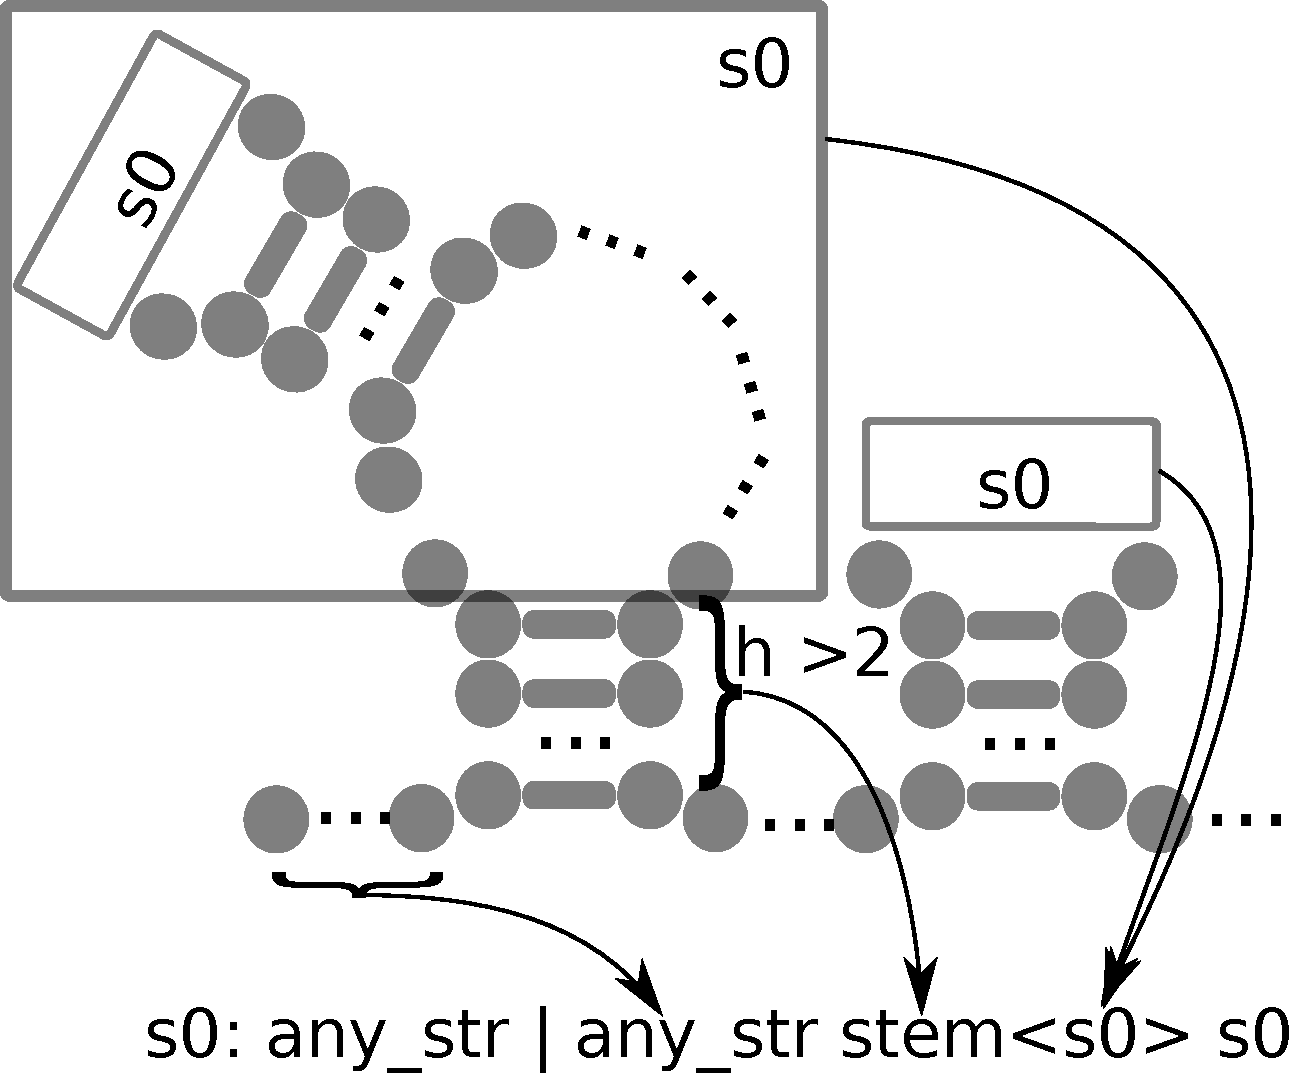
\includegraphics[width=.45\textwidth]{figures/16sgrammar.pdf}
\caption{The graphical explanation of the pattern specified by the grammar $G_0$ in figure~\ref{fig:cfg-rna}}
\label{fig:cfg-rna-graphical}
\end{figure}

Note, that grammar is a variable parameter of our solution and may be tuned for specific cases.
The grammar presented above is a result of a set of experiments, so there is no reason to state that it is the best grammar for secondary structure features extraction.
For example, one can vary the length of the unfoldable sequence by changing the rule for \verb|any_str|: \verb|any_str : any_smb*[0..10]|, \verb|any_str : any_smb*[1..8]|, or something else.
Also, one can increase (or decrease) the minimal height of stem or add some new features, such as pseudoknots, to the grammar (in case one uses conjunctive grammars instead of the context-free).


\subsection{Parsing Algorithm}

\noindent Parsing is used to determine if the given sequence can be derived in the given grammar.
Additionally, when the sequence is derivable, a derivation tree may be provided as a result of parsing. 
It is a classical way: there is a huge number of works on modeling the secondary structure of the full sequence of interest by using probabilistic grammars and respective parsing techniques~\cite{knudsen2003pfold,Browny1993StochasticCG,Knudsen2005StochasticCG}.
We propose to use parsing to extract features: rather than checking the derivability of the given string or find the most probable derivation we search for all the derivable substrings of the given string for all nonterminals.

CYK~\cite{Younger1967RecognitionAP} is a well-known classical algorithm for undirected parsing. 
This algorithm and its modifications are traditionally used for PCFG/SCFG processing and, as a result, are used in a number of tools, but they demonstrate poor performance on long sequences and big grammars~\cite{Liu2005}.

An alternative approach is to use the algorithms based on matrix multiplication, such as Valiant's algorithm~\cite{Valiant:1975:GCR:1739932.1740048}.
From the practical standpoint, matrix-based algorithms allow to easily utilize advanced techniques, such as algorithms for sparse and boolean matrices, GPGPU-based libraries, etc.

Moreover, the matrix-based approach can be generalized to conjunctive and even boolean grammars~\cite{OKHOTIN2014101}, as far as to multiple context-free grammars~\cite{mcfgMatrices}, which can provide a base for more expressive features descriptions handling without significant changes in other parts of our solution.

In our work, we use a version of the matrix-based algorithm~\cite{Azimov:2018:CPQ:3210259.3210264}.
The theoretical time complexity of this algorithm is worse than the complexity of the Valiant's algorithm, but it demonstrates better performance in practice along with a simpler implementation since this algorithm avoids machinery on submatrices manipulation.

\subsection{Matrices}

\noindent The result of parsing is a set of square boolean matrices. 
Each matrix $M_N$ contains information of all substrings which can be derived from the nonterminal $N$.
In other words, $M_N[i,j]=1$ iff $N \Rightarrow^*_G w[i,j-1]$ where $w$ is the input sequence and $G$ is a context-free grammar, and $N$ is a nonterminal.
Thus, the result of parsing is a set of matrices: one matrix for each nonterminal from the grammar.
For further processing, we can select nonterminals of interest.
In our case, for grammar $G_0$, we select the matrix for the nonterminal \verb|s1|.

\begin{figure}
\centering
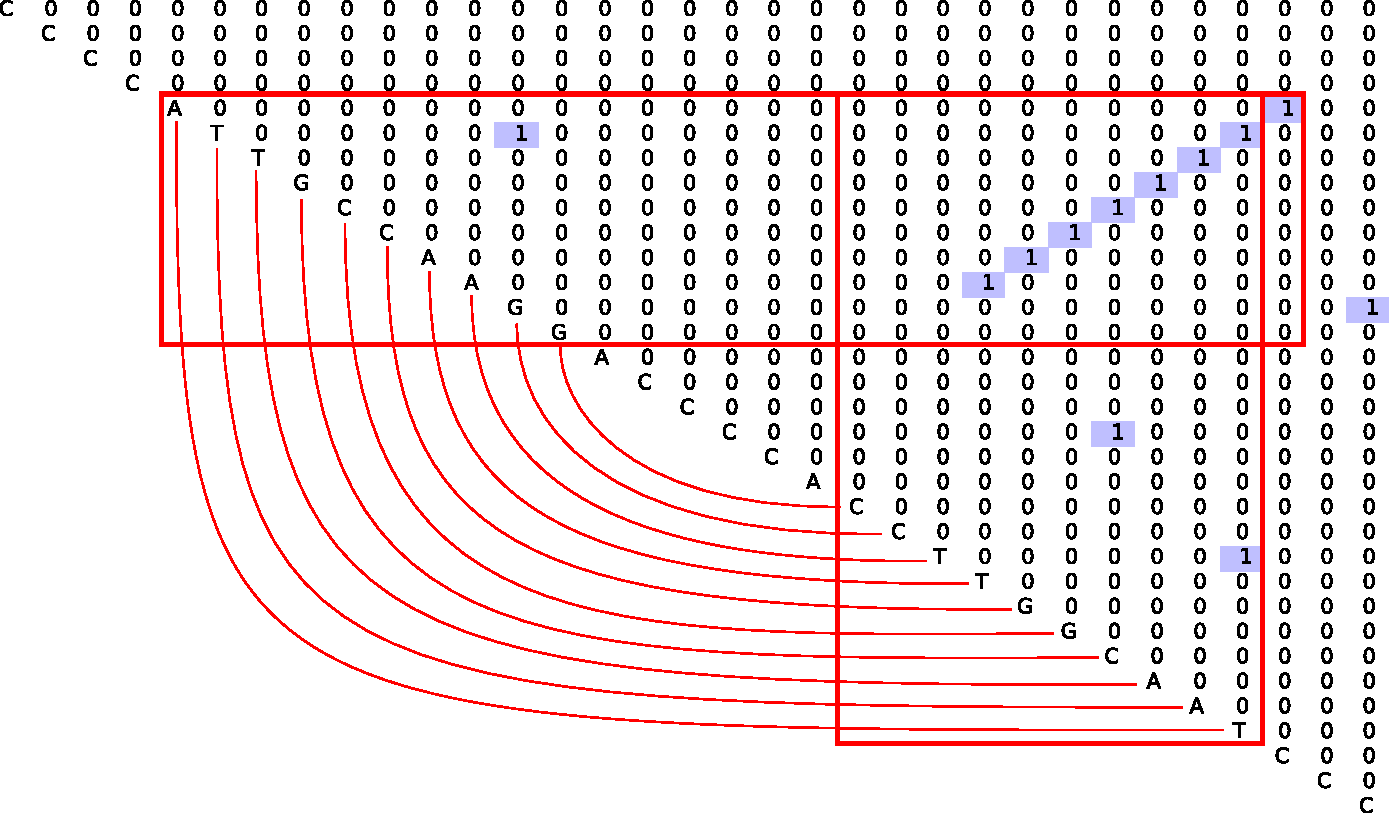
\includegraphics[width=.45\textwidth]{figures/4.pdf}
\caption{Parsing result for sequence which should folds to stem}
\label{fig:matrix-simple-stem}
\end{figure}

The example of such matrix is provided in figure~\ref{fig:matrix-simple-stem}.
This matrix is a result of parsing of the sequence { \center{$w_1=$\texttt{CCCCATTGCCAAGGACCCCACCTTGGCAATCCC}} \\} w.r.t the grammar $G_0$.
One can see an upper right triangle of the parsing matrix (bottom left is always empty, so omitted) with input string on the diagonal.
Note that the string is added only for example readability and a real matrix does not contain the input string, only results of its parsing.
Each filled cell $[i,j]$ which contains 1 denotes that the subsequence $w_1[i,j-1]$ is derivable from \verb|s1| in $G_0$ (so, this subsequence folds to a stem of height 3 or more).
In order to find stems with the height of more than 3, one should detect diagonal chains of 1-s: in our example the stem is of height 10, and one can find chain of 1-s of the length $8=10-2$ (first 1 is a root of the stem of height 3, and each next 1 is a new base pair upon this stem --- root of the stem with height increased by one).
Red boxes and contact map are added for navigation simplification.

Our goal is to extract all the features of the secondary structure, so, our parser finds all the substrings which can be derived from \verb|s1|.
As a result, there are some 1-s out of the chain.
These are correct results: corresponded subsequences can be derived from \verb|s1|. 
In the current example, these 1-s may be treated as noise in some sense, but such behavior may be useful in some cases, as we show later.
Moreover, for long sequences with the complex structure, it may be not evident, which features of the secondary structure are most important.

We use these matrices as an input for the artificial neural network which should detect sufficient features (long chain in our example) and utilize them for applied problem solution (sequence detection or classification, for example).
We drop out the bottom left triangle and vectorize matrices row-by-row to get a bit vector, then convert it to a byte vector and use it as an input.
The transition from bit vector to byte vector is done in order to decrease the input size which is critical for long sequences. 
On the other hand, such operation may significantly complicate network architecture and training, and it is a reason to try to use bitwise networks~\cite{DBLP:journals:corr:KimS16} in the future.  

\subsection{Artificial Neural Networks}

\noindent Artificial neural networks are one possible choice for different classification problems  when data has a hard-to-formalize principal for problem features and contains noise.
Different types of networks suit for images, speech, and natural languages processing.

Classical scenario for classification problems is to provide features vectors and to classify them, meaning that the network can select important features for each required class.
In our case, the fact that $w[i,j-1]$ is derivable from nonterminal $N$ is a feature.
These facts are encoded in the parsing matrix.
So, the vectorized matrix is a vector of features which is a typical input for a neural network.

We use dense neural network because data locality is broken during vectorization and any convolutions are inapplicable.
Moreover, convolutions are used mostly for features extraction, but in our case features are already extracted by parsing.
Thus we need only to detect principal features and relations between them.
It is best done with dense networks.

One of the problems with arbitrary data processing by using neural networks is the input size normalization.
The input layer of the network has fixed size, but input sequence length and hence the length of vectorized parsing result may vary even for the fixed task.
For example, if we want to create a solution for tRNA processing, we should handle sequences of the length approximately from 59 up to 250.
We propose two possible ways to solve this problem.
The first way is subsequences processing: for some tasks, it may be enough to process not a full sequence, but only its subsequence.
In this case, we can set the length of subsequence lower than the shortest sequence which we want to handle. 
This way is useful for long sequences processing (16s rRNA, for example) but cannot be applied for short sequences processing because of the information loss.
The second way is to set an upper bound and fill the gap with special symbols.
For example, while handling tRNAs we can set the input length to 250, and when we want to process sequence of length 60, then we should fill the rest 190 places by selected special symbol.

The example of the neural network which we use is presented in figure~\ref{fig:nn}.
We actively use dropout and batch normalization because network should perform a number of nontrivial transformations: decompress data from bytes and prepare normalized input which requires additional power.
Although initially, batch normalization is an alternative for dropout~\cite{DBLP:journals:corr:IoffeS15}, we use both of them together because separate use has no effects.

\section{Examples}
\label{sec:examples}

\noindent Here we provide more examples of matrices and point out some observations about it in order to provide better intuition of our idea.

\begin{figure}
\centering
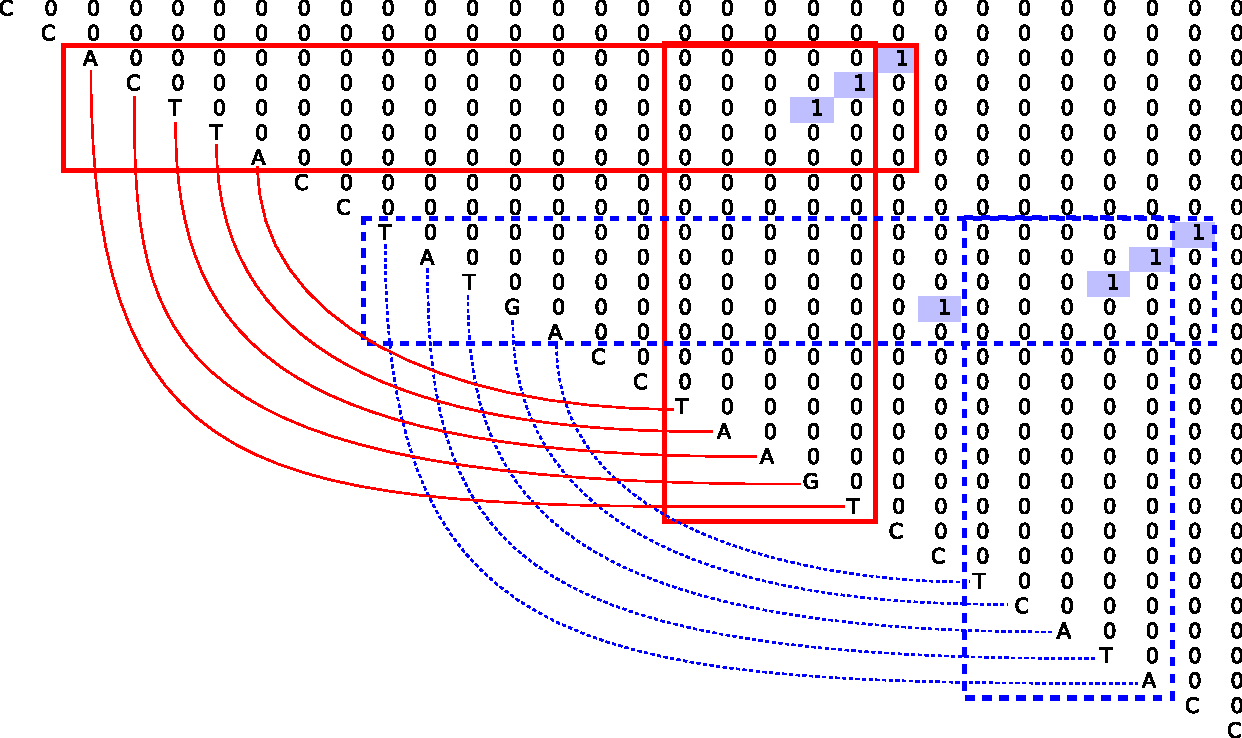
\includegraphics[width=.45\textwidth]{figures/5.pdf}
\caption{Parsing result for sequence which should folds to pseudoknot}
\label{fig:pseudoknot}
\end{figure}

The first part is the observation about pseudoknots. 
Let consider the following sequence which can fold to pseudoknot as an example: {\center{$w_2=$\texttt{CCACTTACCTATGACCTAAGTCCTCATACC.}\\}}
Note, that this sequence is synthetic.
As mentioned above, pseudoknots cannot be expressed in terms of context-free grammars. 
But one can think of a pseudoknot as two crossing stems, and the parser can extract both of them, as presented in figure~\ref{fig:pseudoknot}.
So,~if a neural network is powerful enough, it can detect that if these two features appear simultaneously, then the sequence contains pseudoknot.
As a result, we can detect features which are not expressible in context-free grammars.

The second is an example of a matrix for the real tRNA.
Parsing result of the tRNA\footnote{The sequence Novosphingobium\_aromaticivorans\_DSM\_12444\_chr.trna57-GlyGCC (268150-268084)  Gly (GCC) 67 bp Sc: 22.97. From GtRNAdb: \url{http://gtrnadb2009.ucsc.edu/download.html}. Access date: 02.11.2018.} sequence {\center{$w_3=$\texttt{CAGGGCATAACCTAGCCCAACCTTGCCAAGG \\ 
 TTGGGGTCGAGGGTTCGAATCCCTTCGCCCGCTCCA} \\ }} is presented in figure~\ref{fig:real-trna}. Also, one can see predicted secondary structures\footnote{Predicted secondary structures are given by using the Fold Web Server with default settings: \url{http://rna.urmc.rochester.edu/RNAstructureWeb/Servers/Fold/Fold.html} Access date: 02.11.2018.} (top two) in figures~\ref{fig:real-trna-folding1} and~\ref{fig:real-trna-folding2}.

\begin{figure}
\centering
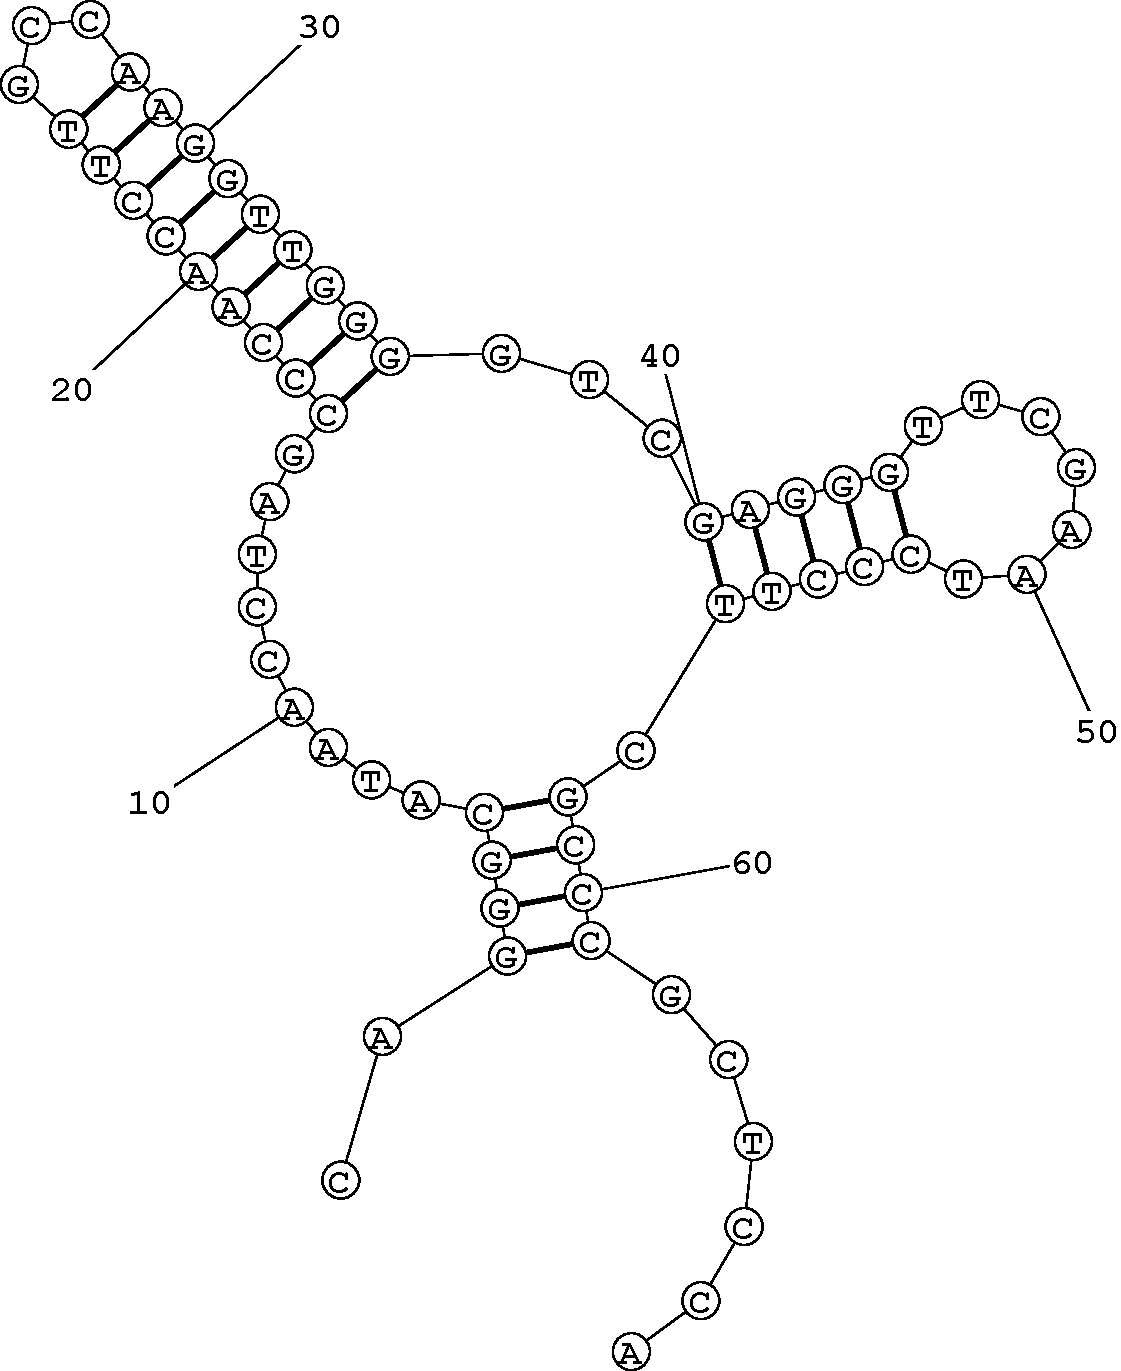
\includegraphics[width=.45\textwidth]{figures/Fold1.pdf}
\caption{Predicted secondary structure for $w_3$}
\label{fig:real-trna-folding1}
\end{figure}


\begin{figure}
\centering
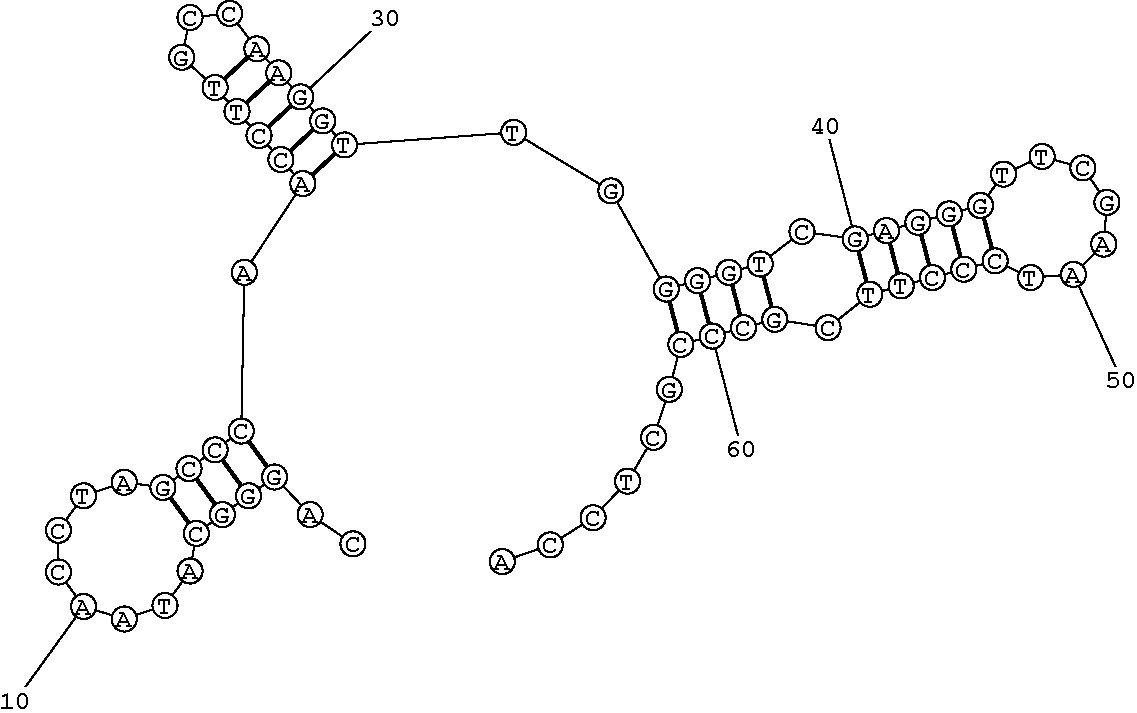
\includegraphics[width=.45\textwidth]{figures/Fold2.pdf}
\caption{Predicted secondary structure for $w_3$}
\label{fig:real-trna-folding2}
\end{figure}

Colored boxes in figure~\ref{fig:real-trna} marks features which correspond to these two predicted foldings: blue dashed marks for~\ref{fig:real-trna-folding1} and red for~\ref{fig:real-trna-folding2}.
Note, that our grammar $G_0$ handles only classical base pairs, so the pair \verb|G - T| which exists in predicted foldings, is not presented in parsing result.
Anyway, we can see that all expected information on the secondary structure is presented in the matrix with some additional features, of course.
And it is a field for neural networks --- to select appropriate features.

\begin{figure*}
\centering
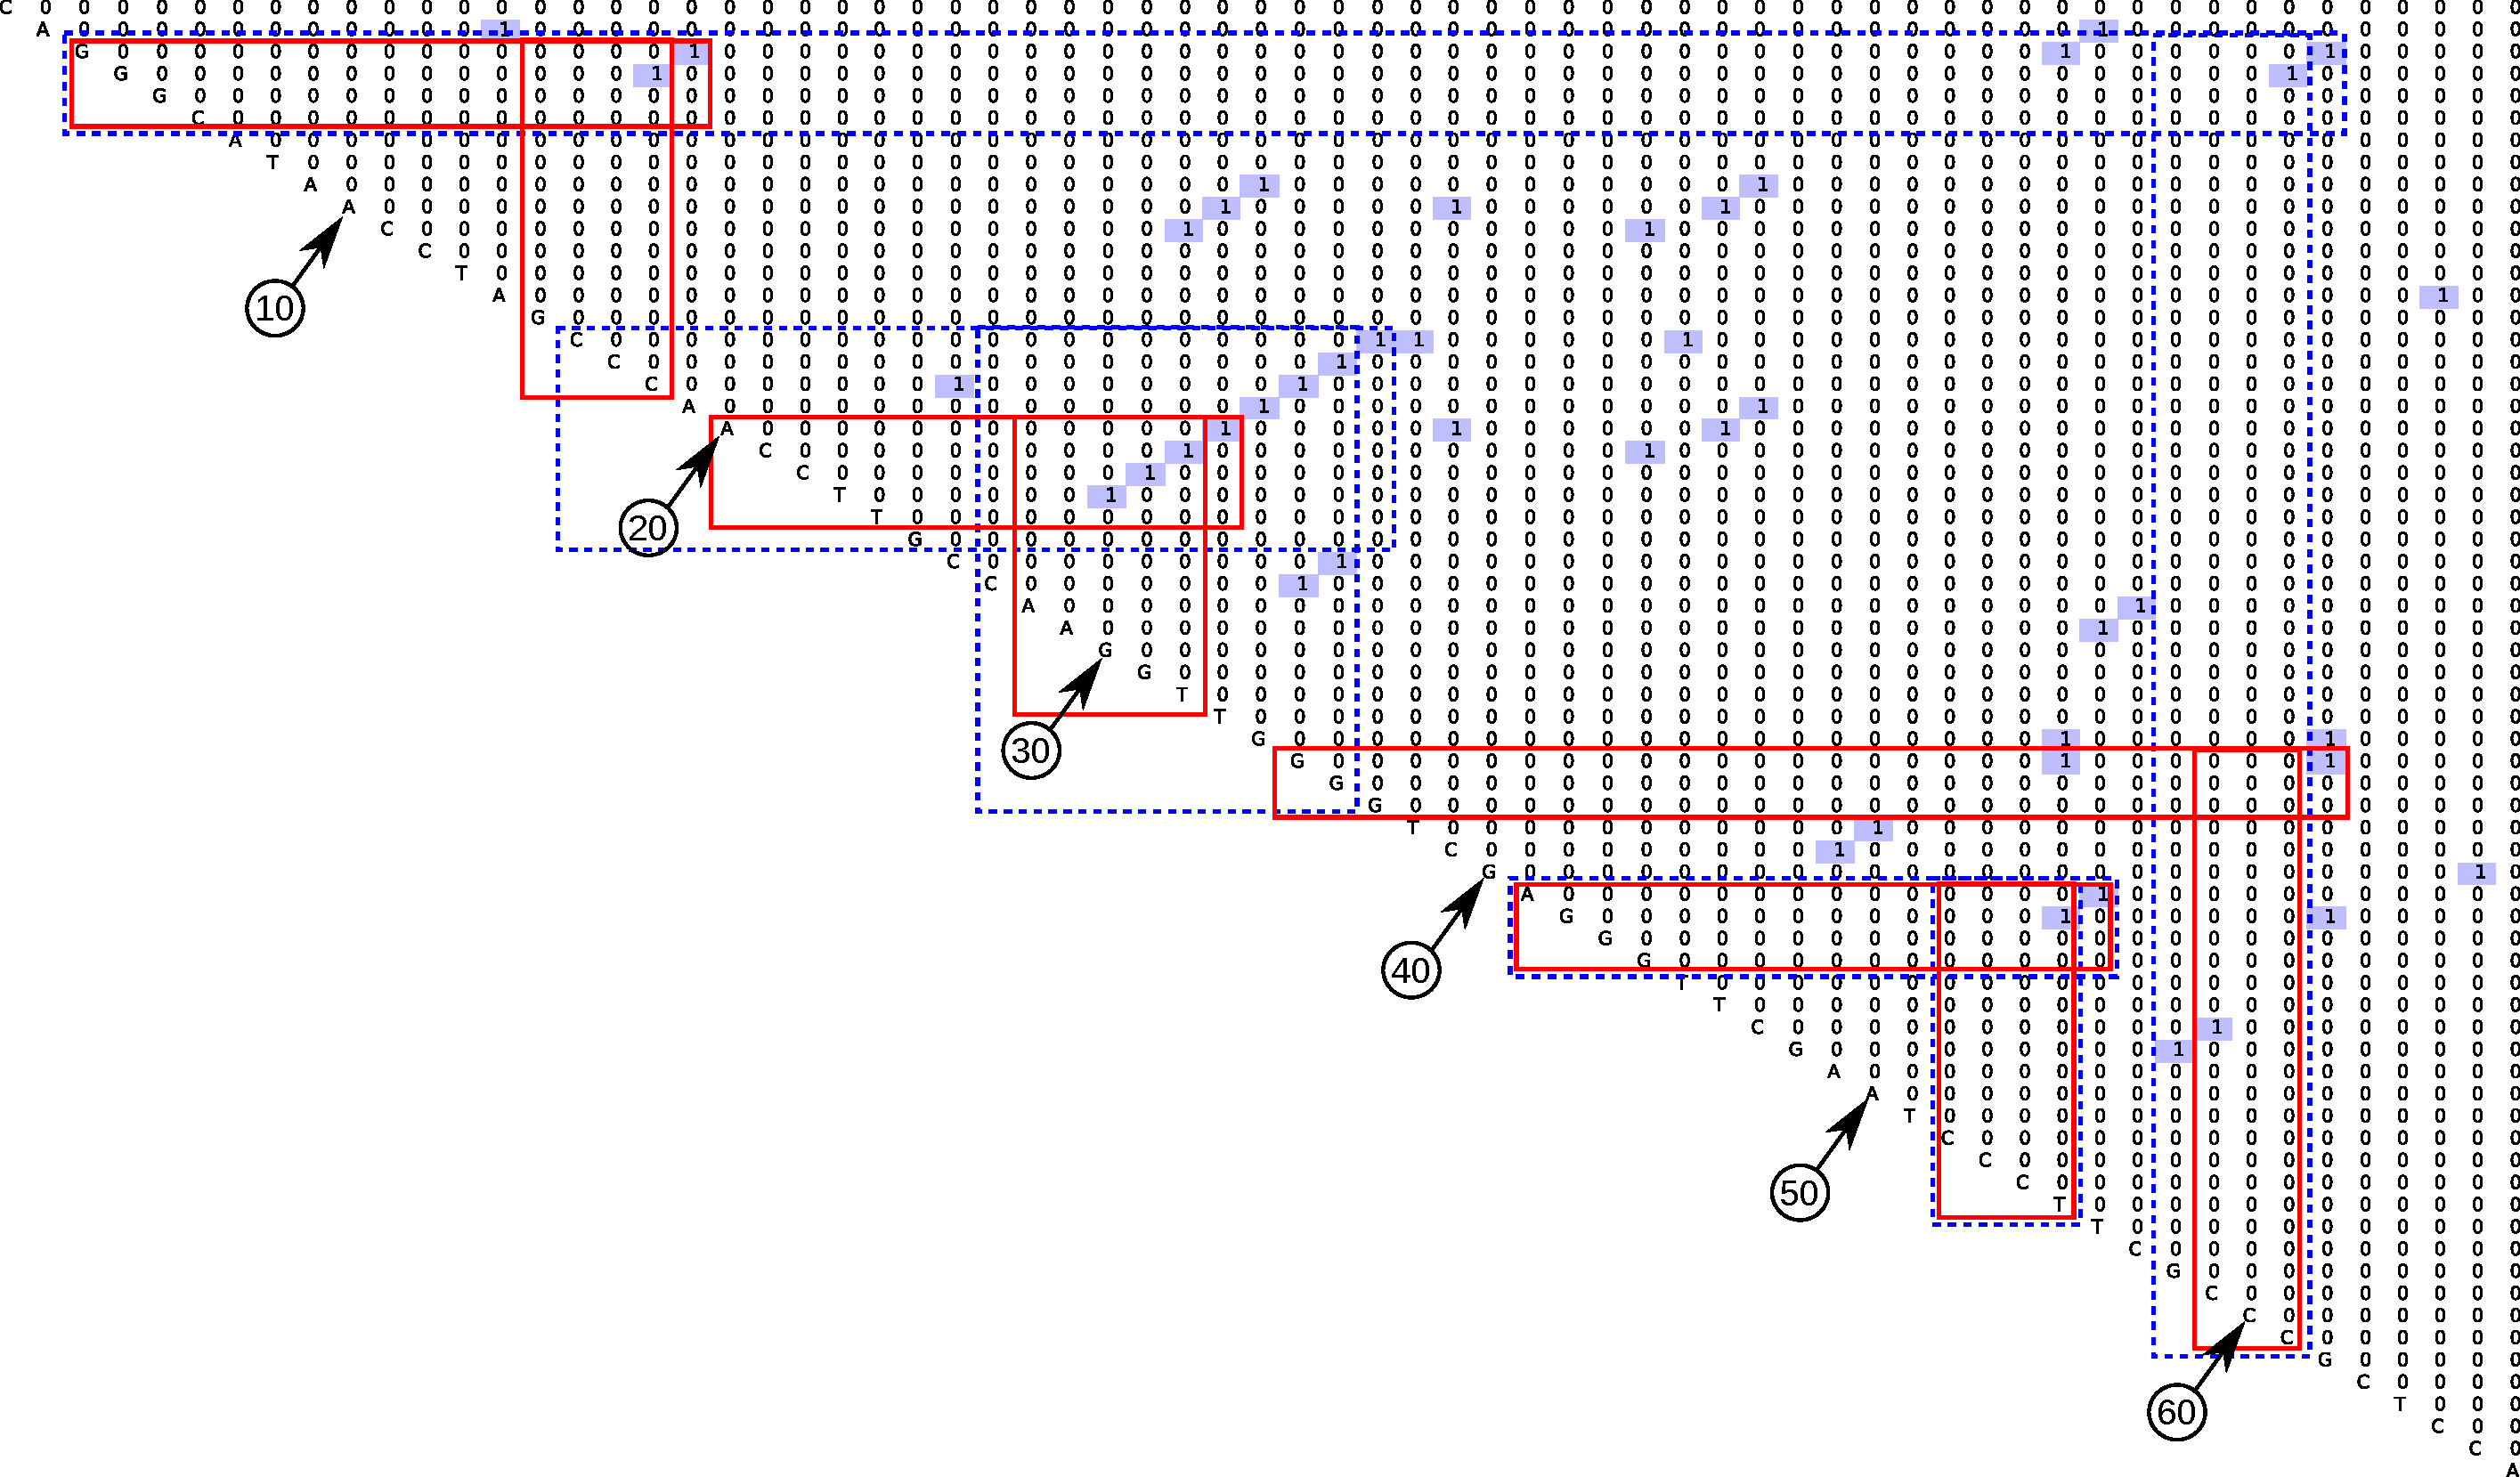
\includegraphics[width=.98\textwidth]{figures/0m.pdf}
\caption{Parsing result for the real tRNA ($w_3$)}
\label{fig:real-trna}
\end{figure*}

We conclude that powerful enough neural networks may detect very nontrivial compositions of secondary structure features. 
What kinds of applications may be built by using such results is an interesting question for future research.

\section{\uppercase{Evaluation}}
\label{sec:evaluation}

\noindent We evaluate the proposed approach on two cases: 16s rRNA detection and tRNA classification.
Note that the goal of the evaluation is to demonstrate the applicability of the approach described above.
We do not provide a comparison with existing tools because our solution is a prototype.
All of these are future work.

\subsection{16s rRNA Sequences}
\noindent The first problem is 16s rRNA detection.
We specify context-free grammars which detect stems with the height of more than two pairs and their arbitrary compositions (namely, $G_0$).
For network training, we use a dataset consisting of two parts: random subsequences of 16s rRNA sequences from the Green Genes database~\cite{pmid16820507} form positive examples, while the negative examples are random subsequences of full genes from the NCBI database~\cite{pmid19854944}.
All sequences have the length of 512 symbols, totally up to 310000 sequences.
After training, current accuracy is 90\% for validation set (up to 81000 sequences); thus we conclude that our approach is applicable.

\subsection{tRNA Sequences}

\noindent The second problem is tRNA classification: we train a neural network to separate tRNAs into two classes: prokaryotes and eukaryotes.
We prepare 50000 sequences from GtRNADB~\cite{Chan2009} for training: 35000 for training and 15000 for testing.
In this case, we use the next trick for data size normalization.
We set the upper bound of sequence length to 220 and after that, we align the real tRNA sequence $w$ in the following way: the first $k$ symbols of the input are $w$ ($|w|=k$) and the rest $220-k$ symbols are filled by \verb|$| --- a special symbol which is not in input alphabet.

Also, we prepare the validation set which contains 217984 sequences for prokaryotes and 62656 sequences for eukaryotes.
All data for validation was taken from tRNADB-CE\footnote{tRNADB-CE: \url{http://trna.ie.niigata-u.ac.jp/cgi-bin/trnadb/index.cgi}. Access date: 31.10.2018}~\cite{Abe2010}.

The architecture of the network which we use in this experiment is presented in figure~\ref{fig:nn}.
Note that it is a training configuration: it contains dropout and batch normalization layers which will be removed after training.
This network contains six dense layers and uses \verb|relu| and \verb|sigmoid| activation functions.

\begin{figure}
\centering
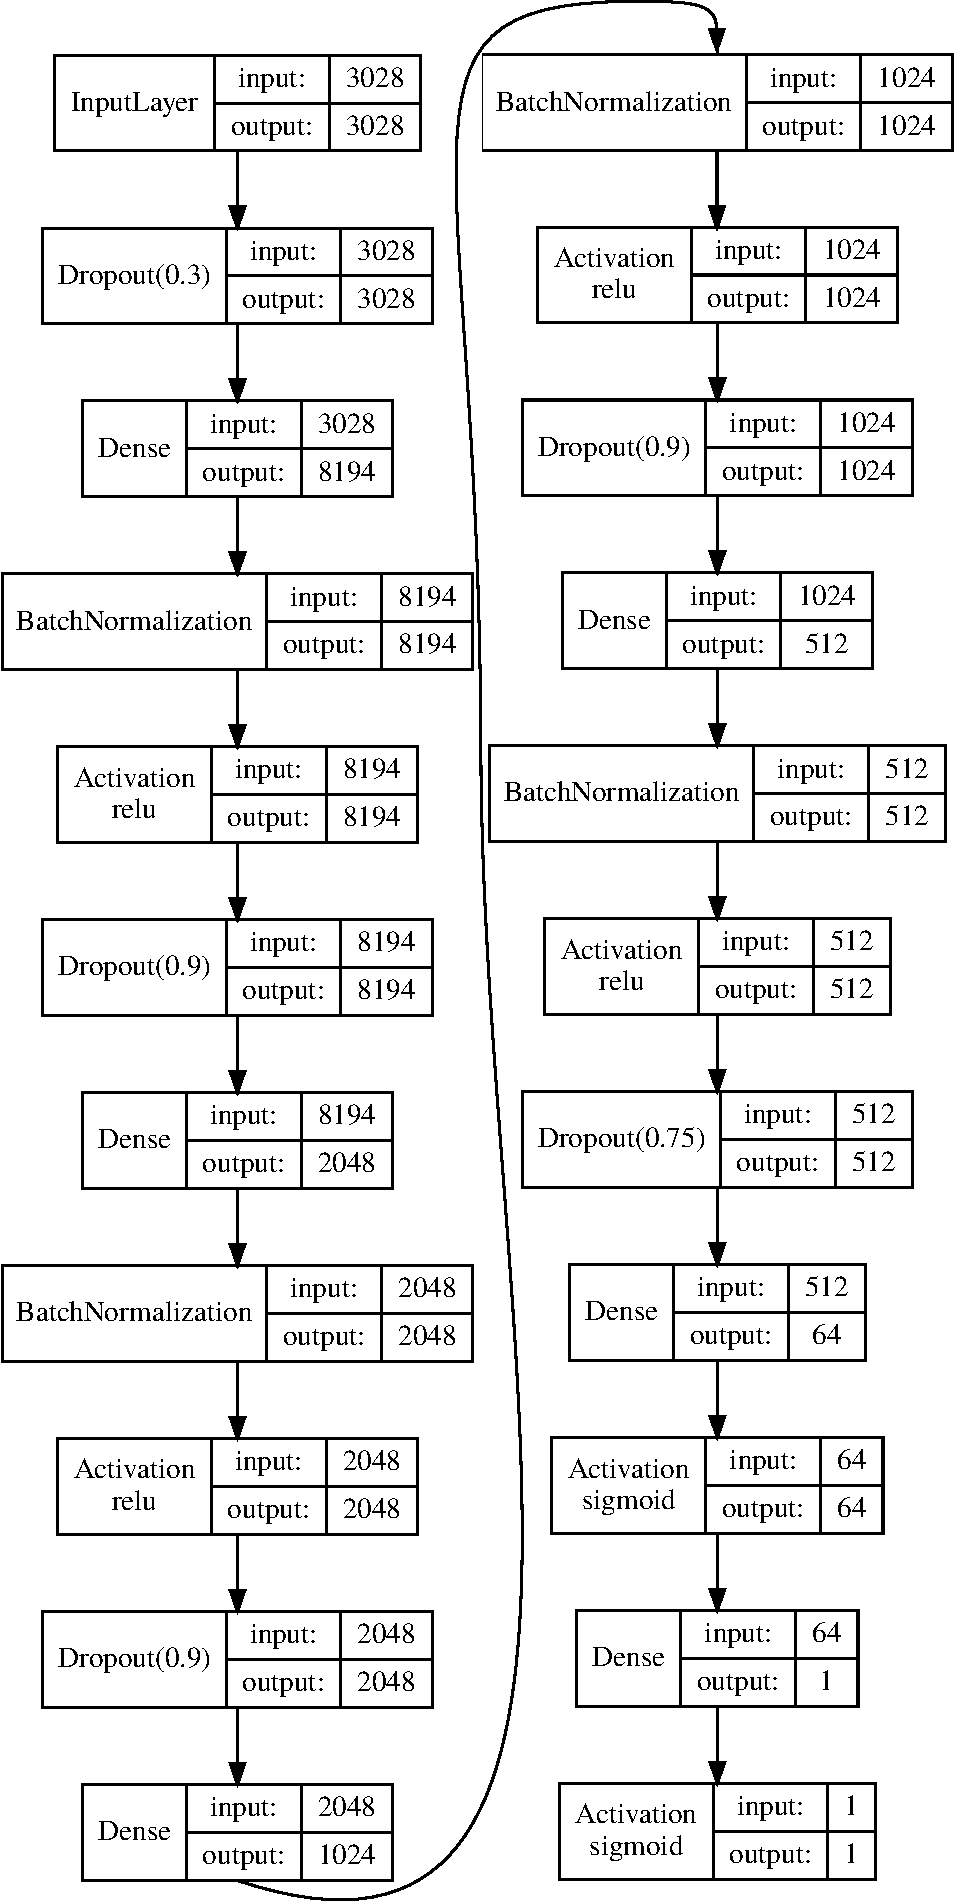
\includegraphics[width=.4\textwidth]{figures/model-crop.pdf}
\caption{architecture of the neural network for tRNA classification}
\label{fig:nn}
\end{figure}

After training, our network demonstrates the accuracy of 97\%. 
For the validation set, we get the following results: 3276 of eukaryotes (5.23\% of all eukaryotes in the validation set) are classified as prokaryotes and 4373 of prokaryotes (2.01\% of all prokaryotes in the validation set) are classified as eukaryotes. 

We conclude that input normalization by filling sequence to the upper bound of length with the special symbol is working.
Also, we can state that the secondary structure contains sufficient information for classification.


\section{\uppercase{Discussion}}
\label{sec:Discussion}

\noindent The presented is a work in progress. 
The ongoing experiment is finding all instances of 16s rRNA in full genomes.
Also, we plan to use the proposed approach for the filtration of chimeric sequences and classification.
A composition of our approach with other methods and tools as well as grammar tuning and detailed performance evaluation may improve the applicability for the real data processing.

One problem of the proposed approach is that parsing is a bottleneck.
A possible solution is to construct a network which can handle sequences instead of parsing data.
It may be done in the following way.
\begin{enumerate}
\item Create a training set of matrices using parsing.
\item Build and train the network $NN_1$ which can handle vectorized matrices.
\item Create new network $NN_2$ by extending $NN_1$ with a head (set of layers) which should convert the sequence to input for $NN_1$
\item Train $NN_2$. Fix the weights of layers from $NN_1$.
\item For the concrete problem, we can tune weights of $NN_2$ to get an appropriate quality.
\end{enumerate}
This way we can use parsing only for training which is less performance critical step than usage in an application.

Another task is to understand the features which network extracts in order to get inspiration in, for example, grammar tuning.
It may be done by trained network visualization.
There is a set of tools for user-friendly convolutional networks visualization, but not for dense networks.
It may be useful to create such a tool and customize it for our domain.

We do some experiments in genomic sequence analysis, but what about proteomics?
Works on grammar-based approaches to proteomics sequences analysis have a long history~\cite{Jimenez-Montano1984,Dyrka2008ASC,Sciacca2011AnnotatedSC}.
This area provides new challenges, such as more complex grammar, more symbols in the alphabet, more complex rules of interactions, more complex features.
As a result, more powerful languages may be needed in this area.
So, we are curious to apply the proposed approach to proteomics sequences analysis.
One of the possible crucial problems is to detect functionally equivalent sequences with sufficiently different length.

Also, it may be reasonable to use other types of neural networks.
Bitwise networks~\cite{DBLP:journals:corr:KimS16} may be reasonable because the result of parsing is a bitwise matrix, so it looks natural to use these networks to process such result. 
Another direction is convolutional networks utilization.
One can treat parsing matrices as bitmaps: one can set a specific color for each nonterminal and get a multicolor picture as a sum of matrices.
The problem here is a picture size: typical matrix size is $n \times n$ where $n$ is a length of the input sequence.

An important part of work is training data preparation.
One of the difficult problems is the creation of a balanced dataset.
Biological datasets (like GreenGenes) contain a huge number of samples for some well-studied organisms and a very small number of samples for others.
Moreover, datasets often contain unclassified and unconfirmed sequences.
It is not evident how to prepare datasets to get a high-quality trained network.

To conclude, our work is at the beginning stage, but current results are promising. 
There is a huge number of experiments in different directions which have potential.
In order to choose the right direction, we hope to discuss future work with the community.


\section*{\uppercase{Acknowledgements}}

\noindent The research was supported by the Russian Science Foundation grant 18-11-00100 and a grant from JetBrains Research.


\vfill

\bibliographystyle{apalike}
{\small
\bibliography{example}}


\vfill
\end{document}

